\documentclass[letterpaper,10pt]{article}
\usepackage[margin=1in]{geometry}
\usepackage{amsmath,amssymb,booktabs,array,graphicx,float}
\usepackage{subcaption}  % For subfigure environments
\usepackage[font=small,labelfont=normalfont]{caption}
\usepackage[hidelinks]{hyperref}
\setlength{\parindent}{0pt}
\setlength{\parskip}{0.25em}
\setlength{\intextsep}{7pt plus 2pt minus 1pt}
\captionsetup{skip=5pt}
\setlength{\emergencystretch}{2em}
\renewcommand{\arraystretch}{1.14}
\raggedbottom
\makeatletter
\renewcommand\section{\@startsection{section}{1}{0pt}{1.8ex plus .6ex minus .2ex}{.8ex plus .2ex}{\normalfont\Large}}
\renewcommand\subsection{\@startsection{subsection}{2}{0pt}{1.5ex plus .5ex minus .2ex}{.6ex plus .2ex}{\normalfont\large}}
\renewcommand{\maketitle}{\begin{center}{\LARGE\@title\par}\vspace{.5em}\@author\par\vspace{.2em}\@date\end{center}\vspace{.15em}}
\makeatother
\title{Physics 5CL Lab 5 Atomic Spectra}
\author{Isaac Chan and Forrest Chou}
\date{October 2026}
\begin{document}
\maketitle
\section{Experiment 1: Helium}
\subsection{Reference line}

We placed the transmission grating at $45.71\,\text{cm}$ and the spectrometer scale at $9.13\,\text{cm}$, with the discharge tube behind the central opening. Bright first order lines appeared on both sides. A faint second order was visible at large angles, mainly in yellow. We checked alignment by comparing opposite line positions. The apparent line width was about $0.1\,\text{cm}$.

\begin{figure}[H]
\centering
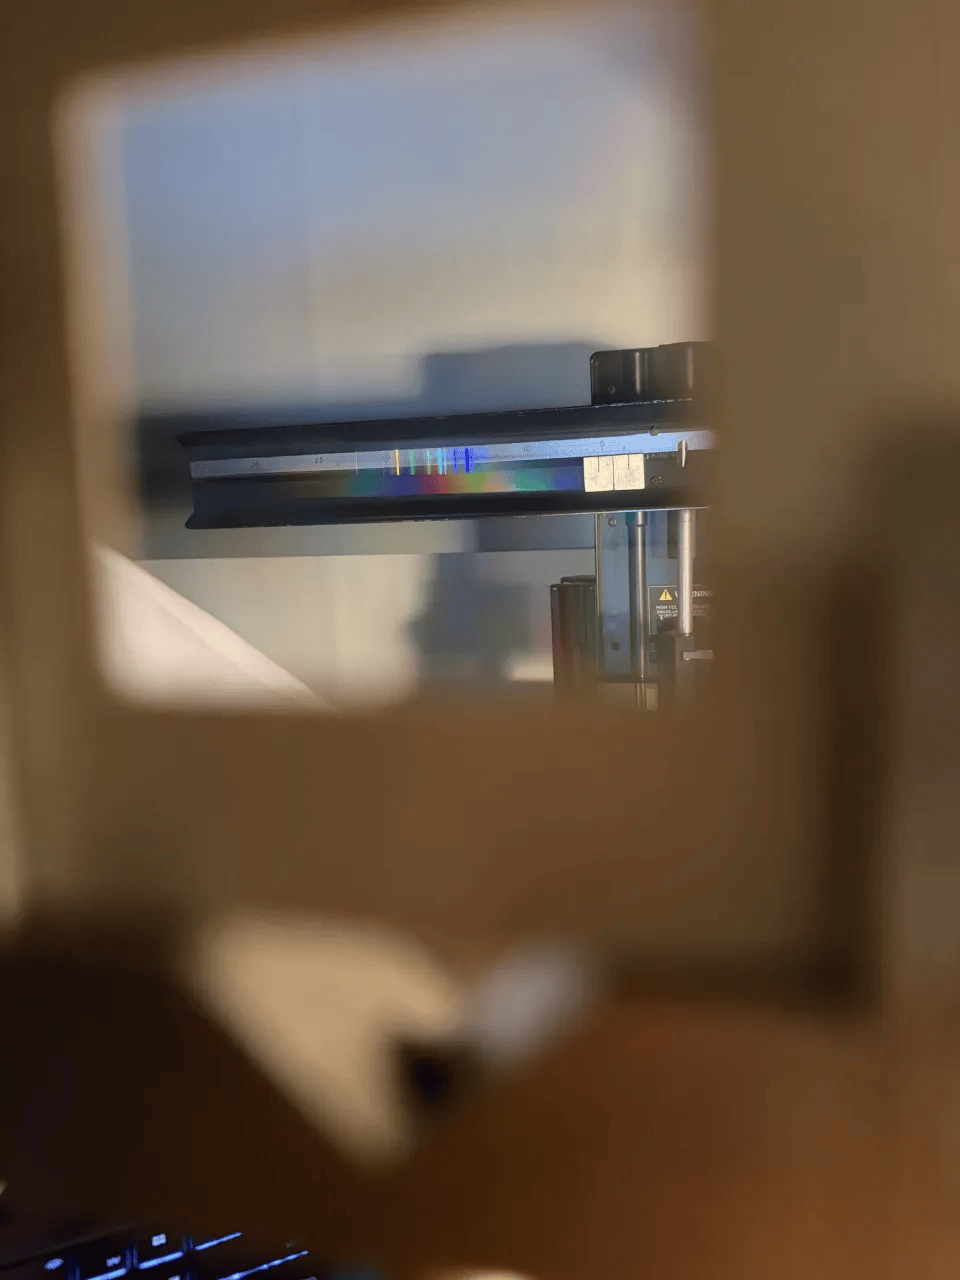
\includegraphics[width=\linewidth,trim=80bp 600bp 180bp 300bp,clip]{Photos/5CL_5_1.png}
\caption{Helium viewed through the transmission grating.}
\label{fig:helium}
\end{figure}

\begin{table}[H]
\centering
\begin{tabular}{cccc}
\toprule
Observer & Left / $\text{cm}$ & Right / $\text{cm}$ & Recorded uncertainty / $\text{cm}$ \\
\midrule
Isaac & 11.18 & 11.11 & 0.15 \\
Forrest & 11.30 & 11.30 & 0.10 \\
\bottomrule
\end{tabular}
\caption{Independent placements of the helium D3 line. The uncertainty column preserves the original estimates. Experiment 2 uses the measured scatter of these four readings.}
\label{tab:helium-repeat}
\end{table}

\clearpage
\subsection{Visible spectrum}

We recorded three additional first order lines on the right. Using the known D3 wavelength $587.6\,\text{nm}$ and the full grating geometry gives
\begin{equation}
\lambda=d\sin\theta=d\frac{y}{\sqrt{L_{He}^2+y^2}}.
\end{equation}

\begin{table}[H]
\centering
\begin{tabular}{ccc}
\toprule
Observed color & Recorded $y$ / $\text{cm}$ & Calculated $\lambda$ / $\text{nm}$ \\
\midrule
Red & $12.87\pm0.09$ & $665\pm5$ \\
Yellow (D3) & $11.22\pm0.05$ & 587.6 (reference) \\
Green & $9.51\pm0.09$ & $504\pm5$ \\
Blue & $8.46\pm0.09$ & $451\pm5$ \\
\bottomrule
\end{tabular}
\caption{Calculated helium wavelengths, with uncertainties propagated by the method in Experiment 2. The yellow offset is the mean of four placements, and its wavelength is fixed by the reference.}
\label{tab:helium-wavelength}
\end{table}

These roughly match the handout's helium lines near $668\,\text{nm}$ and $588\,\text{nm}$, together with $502\,\text{nm}$ and $447\,\text{nm}$. Strong yellow accompanied by blue and green provides a useful helium fingerprint.

The reflection grating and screen were off the bench, making distances poorly constrained. We used a small reflection angle to reduce projection effects. No additional fluorescence wavelength was recorded.

\begin{figure}[H]
\centering
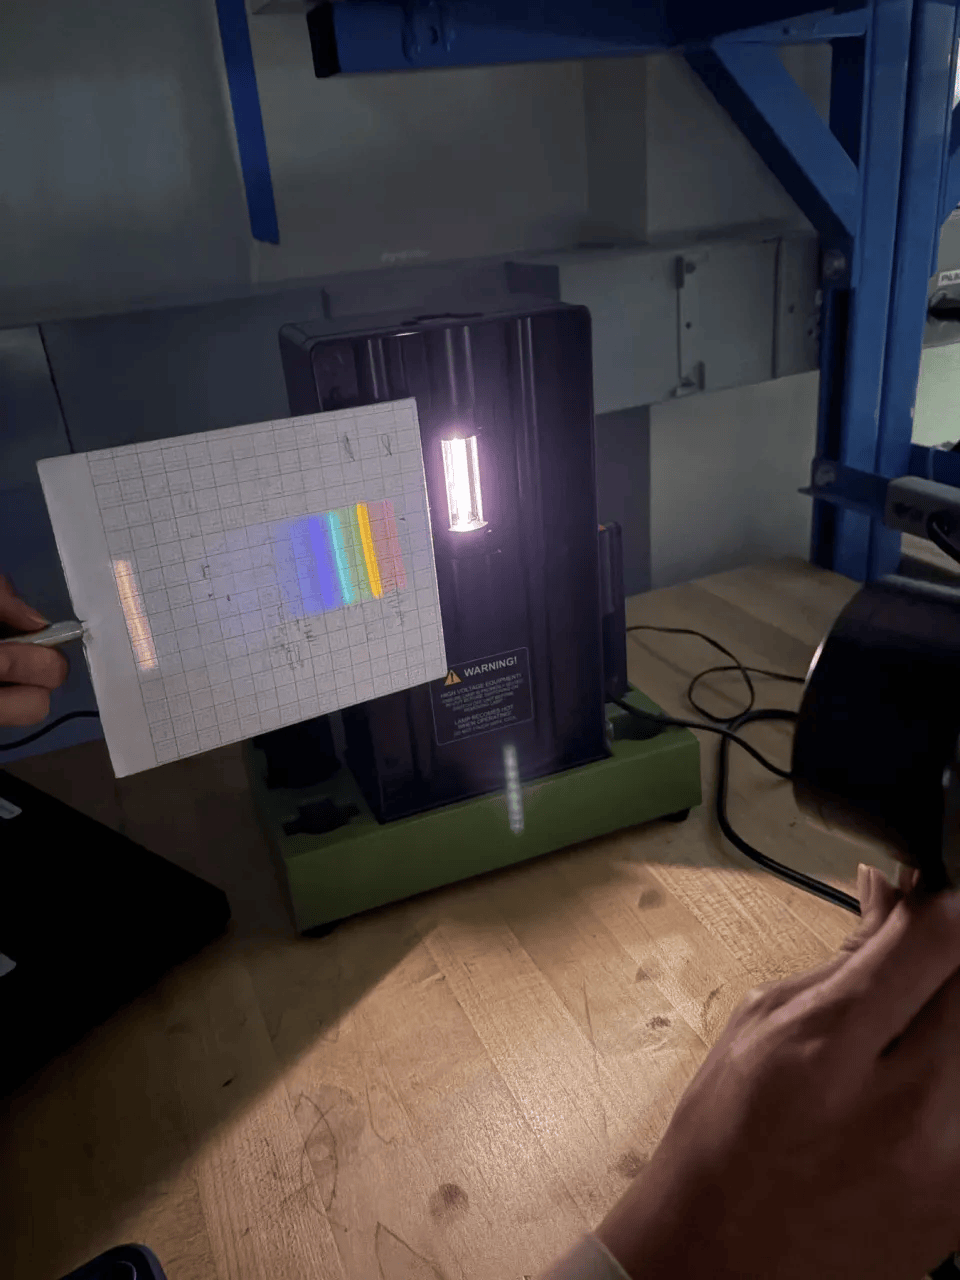
\includegraphics[width=\linewidth,trim=0bp 580bp 60bp 350bp,clip]{Photos/5CL_5_1b.png}
\caption{Helium spectrum projected onto the paper with the reflection grating.}
\label{fig:helium-mirror}
\end{figure}

\clearpage
\section{Experiment 2: Hydrogen}

We use three visible hydrogen lines to test the Balmer relation. The fit gives $R=1.11\times10^7\pm4\times10^5\,\text{m}^{-1}$ and $n_f=2.01\pm0.02$, consistent with the reference Rydberg constant and transitions into the $n=2$ level.

\subsection{Setup and reference measurements}

We placed the hydrogen discharge tube behind the central opening of the spectrometer scale and viewed it through the same transmission grating used for helium. The scale and grating positions were $14.35\,\text{cm}$ and $42.20\,\text{cm}$, giving $L_H=27.85\,\text{cm}$. We measured the apparent first order offsets from the central image. Distinct red, cyan, and blue to violet lines form a useful hydrogen fingerprint.

\begin{figure}[H]
\centering
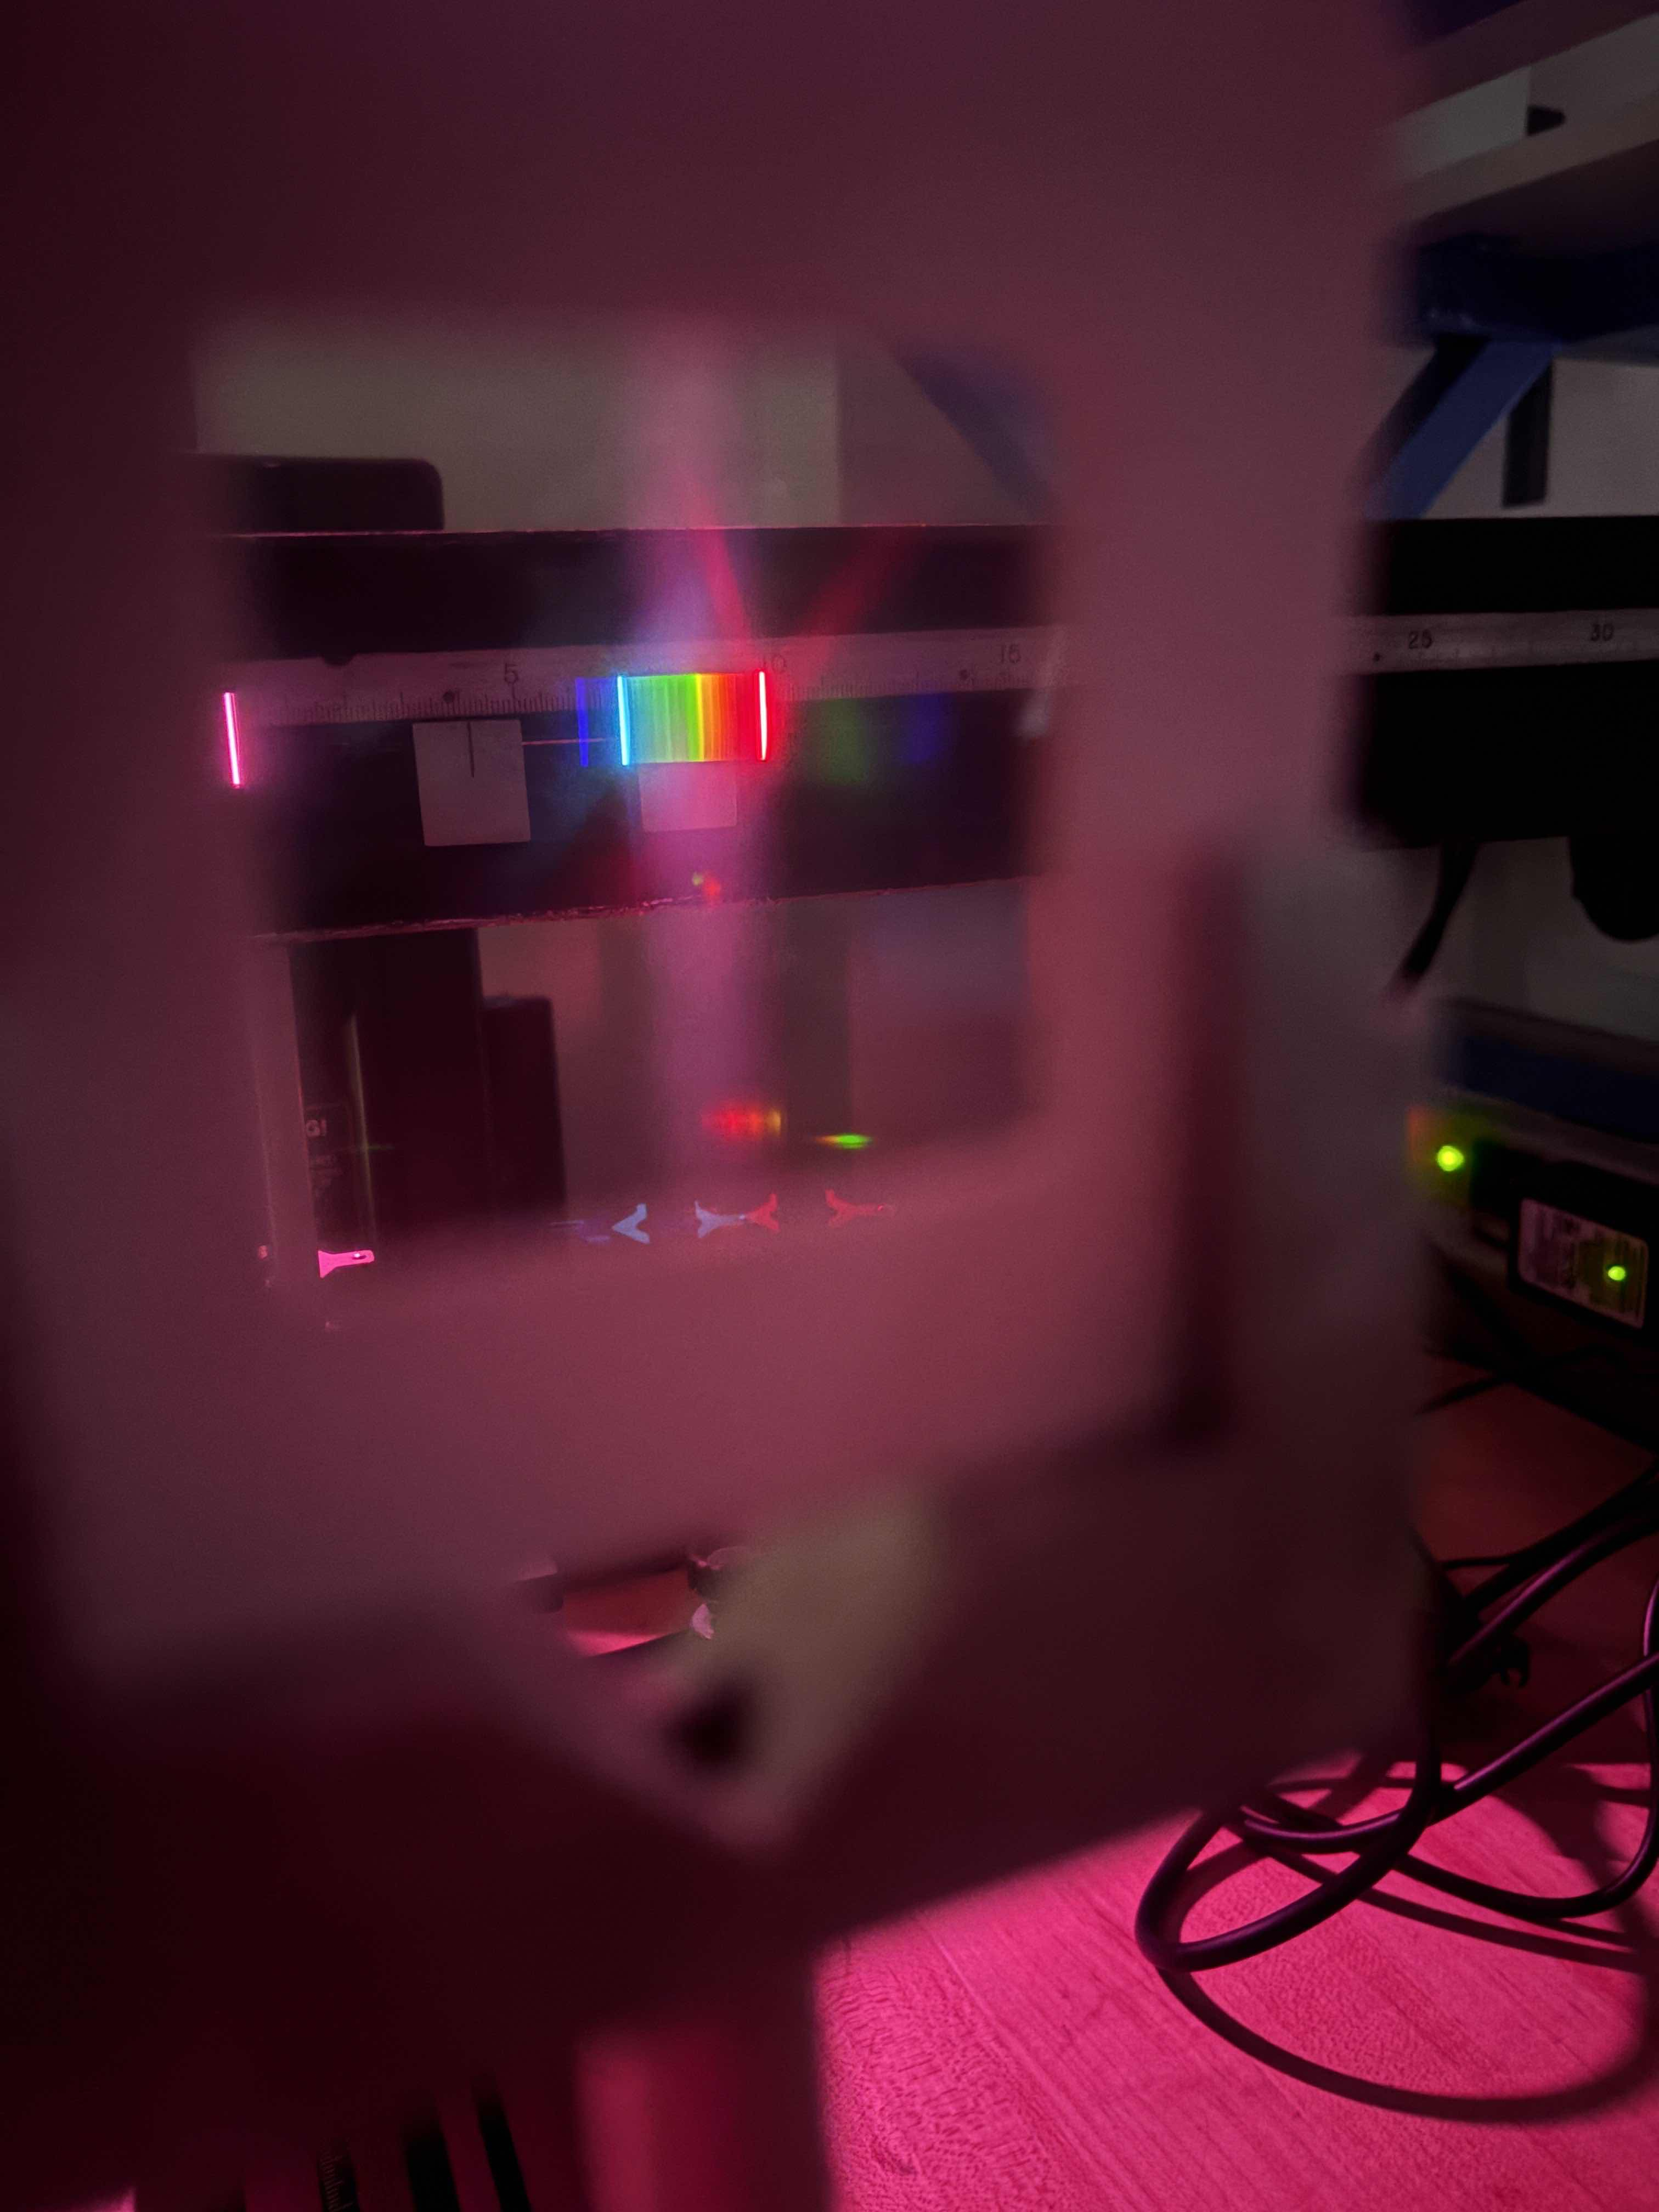
\includegraphics[width=\linewidth,trim=250bp 2432bp 1124bp 1100bp,clip]{Photos/setup2.jpg}
\caption{Hydrogen spectrum viewed through the transmission grating. The prominent lines appear against a broader background. The photograph records the observed pattern, rather than measured line intensities.}
\label{fig:hydrogen-photo}
\end{figure}

\begin{figure}[H]
\centering
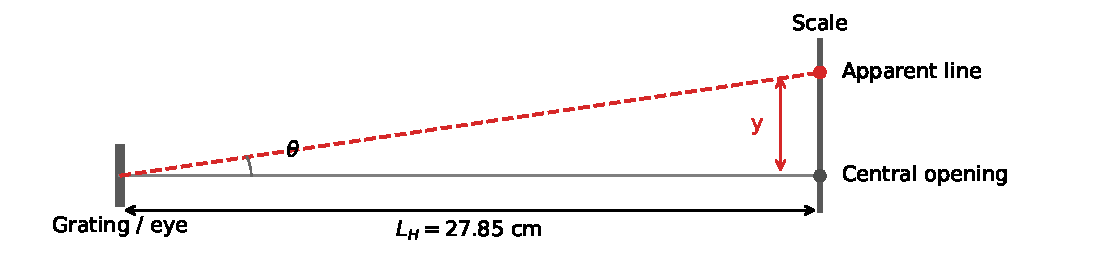
\includegraphics[width=\linewidth]{figures/hydrogen_geometry.pdf}
\caption{Geometry used to convert apparent line position to wavelength. The dashed line is a viewing construction, not a projected beam. The displacement $y$ is measured from the central opening.}
\label{fig:hydrogen-geometry}
\end{figure}

The four helium D3 placements in Experiment 1 give the position statistics
\begin{align}
\bar y_D&=\frac{1}{N}\sum_{j=1}^{N}y_j, \\
s_y^2&=\frac{1}{N-1}\sum_{j=1}^{N}(y_j-\bar y_D)^2, \\
u_D&=\frac{s_y}{\sqrt{N}}.
\end{align}
For $N=4$, we obtain $\bar y_D=11.22\pm0.05\,\text{cm}$, $s_y=0.09\,\text{cm}$, and $u_D=0.05\,\text{cm}$. Following the handout, the standard error $u_D$ describes the mean reference position, while the sample standard deviation $s_y$ describes a new line placement. We retain the unrounded values in all calculations.

\clearpage
\subsection{Wavelengths and propagated uncertainty}

For a first order maximum, the grating equation and viewing geometry give
\begin{align}
\lambda&=d\sin\theta, \\
\sin\theta&=\frac{y}{\sqrt{L^2+y^2}}.
\end{align}
The largest hydrogen angle is about $19^\circ$, so we retain the full geometry. Using $\lambda_D=587.6\,\text{nm}$ and the helium separation $L_{He}=36.58\,\text{cm}$,
\begin{align}
d&=\lambda_D\frac{\sqrt{L_{He}^2+\bar y_D^2}}{\bar y_D}=2003\pm8\,\text{nm}, \\
u_d&=\frac{\lambda_D L_{He}^2}{\bar y_D^2\sqrt{L_{He}^2+\bar y_D^2}}u_D.
\end{align}
The reference wavelength is held fixed. Bench position uncertainties were not recorded, so the quoted uncertainties also hold both separations fixed.

For a hydrogen position $y$,
\begin{align}
\lambda&=d\frac{y}{\sqrt{L_H^2+y^2}}, \\
u_\lambda^2&=\left(\frac{\lambda}{d}u_d\right)^2+
\left(\frac{dL_H^2}{(L_H^2+y^2)^{3/2}}s_y\right)^2.
\end{align}
Position placement contributes about $6\,\text{nm}$ per line, compared with about $2\,\text{nm}$ from the grating spacing. Visual placement therefore dominates the reported uncertainty. The apparent line width of about $0.1\,\text{cm}$ is comparable to the measured position scatter.

\begin{table}[H]
\centering
\begin{tabular}{ccccc}
\toprule
Line & $y$ / $\text{cm}$ & Calculated $\lambda$ / $\text{nm}$ & Predicted / $\text{nm}$ & $Z_\lambda$ \\
\midrule
Red, $3\to2$ & $9.78\pm0.09$ & $664\pm6$ & 656.1 & 1.2 \\
Cyan, $4\to2$ & $6.97\pm0.09$ & $486\pm6$ & 486.0 & 0.06 \\
Blue/violet, $5\to2$ & $6.24\pm0.09$ & $438\pm6$ & 433.9 & 0.63 \\
\bottomrule
\end{tabular}
\caption{Wavelengths and Balmer assignments. Predictions use the handout's Rydberg constant before rounding. Each $Z_\lambda$ is the measured minus predicted wavelength divided by its propagated uncertainty.}
\label{tab:hydrogen-wavelengths}
\end{table}

\begin{figure}[H]
\centering
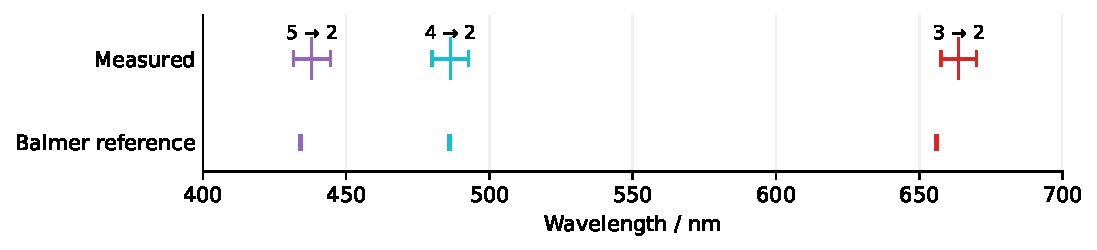
\includegraphics[width=\linewidth]{figures/hydrogen_spectrum.pdf}
\caption{Measured and predicted line positions, labeled by transition. Horizontal bars show wavelength uncertainties. Mark heights are schematic and do not represent measured brightness.}
\label{fig:hydrogen-spectrum}
\end{figure}

The red line has the largest error from the prediction, about $8\,\text{nm}$ or $1.2$ quoted uncertainties. The three lines are compatible with the first three Balmer transitions. Their wavelength ordering and separation also support these assignments. The single line checks are correlated because the same calculated grating spacing enters every wavelength.

\clearpage
\subsection{Bohr fit and statistical interpretation}

Quantized electron energy gaps give the Balmer relation. Defining $x=n_i^{-2}$ and $w=\lambda^{-1}$ makes it linear,
\begin{align}
w&=R(n_f^{-2}-x)=mx+b, \\
R&=-m, \\
n_f&=\sqrt{-\frac{m}{b}}.
\end{align}
We fit all three points with slope and intercept free. The weighted regression retains the common grating contribution to the wavelength covariance. We use $u_R=u_m$ and propagate the full slope and intercept covariance into $u_{n_f}$.

\begin{figure}[H]
\centering
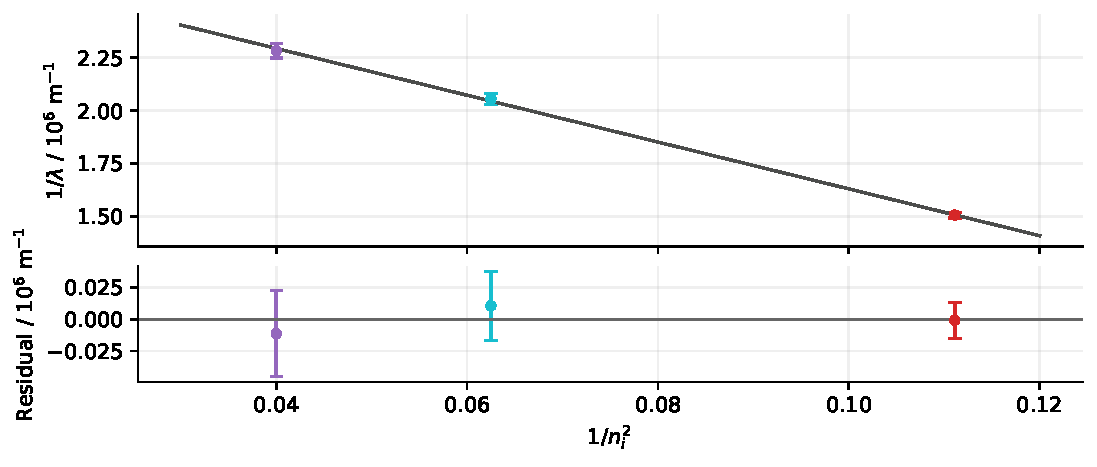
\includegraphics[width=\linewidth]{figures/hydrogen_fit.pdf}
\caption{Reciprocal wavelength fit and raw residuals $w-w_{\text{fit}}$, with the same propagated uncertainties. The quantum numbers are fixed.}
\label{fig:hydrogen-fit}
\end{figure}

\begin{table}[H]
\centering
\begin{tabular}{cccc}
\toprule
Quantity & Calculated result & Reference & Difference / uncertainty \\
\midrule
$m$ / $10^7\,\text{m}^{-1}$ & $-1.11\pm0.04$ & -- & -- \\
$b$ / $10^6\,\text{m}^{-1}$ & $2.74\pm0.04$ & -- & -- \\
$R$ / $10^7\,\text{m}^{-1}$ & $1.11\pm0.04$ & 1.09737 & 0.23 \\
$n_f$ & $2.01\pm0.02$ & 2 & 0.47 \\
\bottomrule
\end{tabular}
\caption{Fit parameters and derived values. The last two rows come from the same fit.}
\label{tab:hydrogen-fit-results}
\end{table}

For residual vector $\mathbf r$ and reciprocal wavelength covariance $C_w$, the fit statistic is
\begin{equation}
\chi^2=\mathbf r^{T}C_w^{-1}\mathbf r.
\end{equation}
The free fit has $\nu=3-2=1$ degree of freedom and $\chi^2=\chi_\nu^2=0.29$, with $p\approx0.59$. Comparing all three wavelengths with the fixed Balmer prediction gives $\chi^2=1.8$ for three degrees of freedom and $p\approx0.62$. Both checks are consistent with the model.

These approximate $p$ values treat the estimated reading errors as fixed Gaussian uncertainties. Four reference placements and one fit residual degree of freedom provide limited evidence about the error scale. We retain the input uncertainties despite the small residuals.

Alignment and unrecorded bench position uncertainty remain possible systematic errors. A common wavelength scale error changes $R$ but cancels from the slope to intercept ratio for $n_f$. Thus $n_f=2$ checks the spectral pattern more directly than the absolute scale. The results support the Balmer model at our precision. A hydrogen reflection grating trace and fluorescence wavelengths were not recorded.

\clearpage
\section{Experiment 3: Mystery Tubes}

Flooding disrupted the first workday, so this experiment followed a modified, qualitative format. We compared the visible patterns of tubes B and C with the candidate gases. We did not collect quantitative spectra for this part, so the identifications below use the recorded color patterns.

\begin{table}[H]
\centering
\begin{tabular}{>{\raggedright\arraybackslash}p{.08\linewidth}>{\raggedright\arraybackslash}p{.43\linewidth}>{\raggedright\arraybackslash}p{.36\linewidth}}
\toprule
Tube & Recorded features & Best qualitative match \\
\midrule
B & Prominent red, orange, and yellow features. & Neon, whose visible spectrum is rich in orange and red lines. \\
C & Many lines, including blue, two distinct green regions, and yellow to red. & Argon, whose lines span a broad range of visible colors. \\
\bottomrule
\end{tabular}
\caption{Observations and candidate identifications. Line positions and relative intensities were not measured.}
\end{table}

Tube B's concentration of prominent warm colored features is consistent with neon. Tube C showed a more varied pattern across the visible range, which is consistent with argon. These comparisons use the handout's descriptions and the \href{https://physics.nist.gov/PhysRefData/Handbook/Tables/neontable2.htm}{NIST neon} and \href{https://physics.nist.gov/PhysRefData/Handbook/Tables/argontable2.htm}{argon line tables}.

The third candidate, molecular nitrogen, can also produce a complex spectrum. Its rotational and vibrational structure creates groups of closely spaced transitions that appear as bands. The notes do not resolve that band structure, so the argon identification is less secure than a match using measured wavelengths.

The spectral pattern carries more information than the overall glow of a tube. A discharge excites the gas, and emitted photon energies reflect differences between its energy levels,
\begin{equation}
\frac{hc}{\lambda}=E_i-E_f.
\end{equation}
Different gases have different energy spacings, so the combination of spectral features acts as a fingerprint. Our observations favor B as neon and C as argon, with the confidence limited by the qualitative comparison.

\clearpage

\section{Experiment 4: Light Bulbs}
\subsection{Procedure}

We observe the spectra of a compact fluorescent and an incandescent light bulb. We expect the different mechanisms of the bulbs to result in different spectral patterns. Due to time constraints in the lab, we report only qualitative findings.

\subsection{Observations}

For the CFL bulb, we observe numerous bright spectral features, particularly the bright red, green, and blue lines, and notice an overall smearing of the spectrum. These features are consistent with a mercury vapor CFL.

We repeat this setup for the incandescent light and observe a smooth spectrum of colors. The hot filament produces a continuous thermal spectrum across the visible range. Red and green appear strongest, and the violet end fades more quickly than the red.

\begin{figure}[H]
\centering
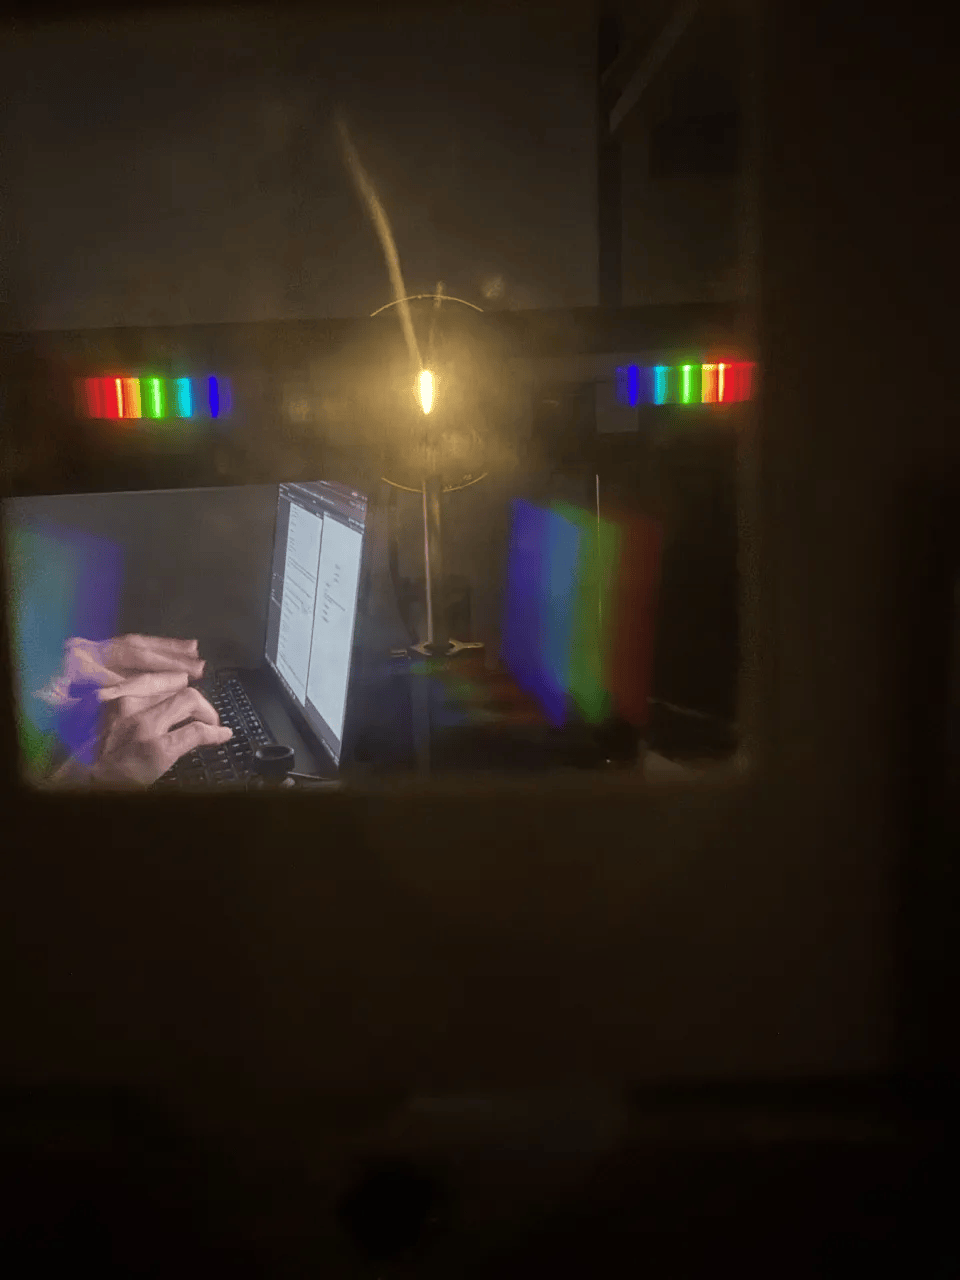
\includegraphics[width=\linewidth,trim=80bp 750bp 80bp 250bp,clip]{Photos/5CL_5_4a.png}
\caption{CFL spectrum with bright lines and overall smearing.}
\end{figure}

\begin{figure}[H]
\centering
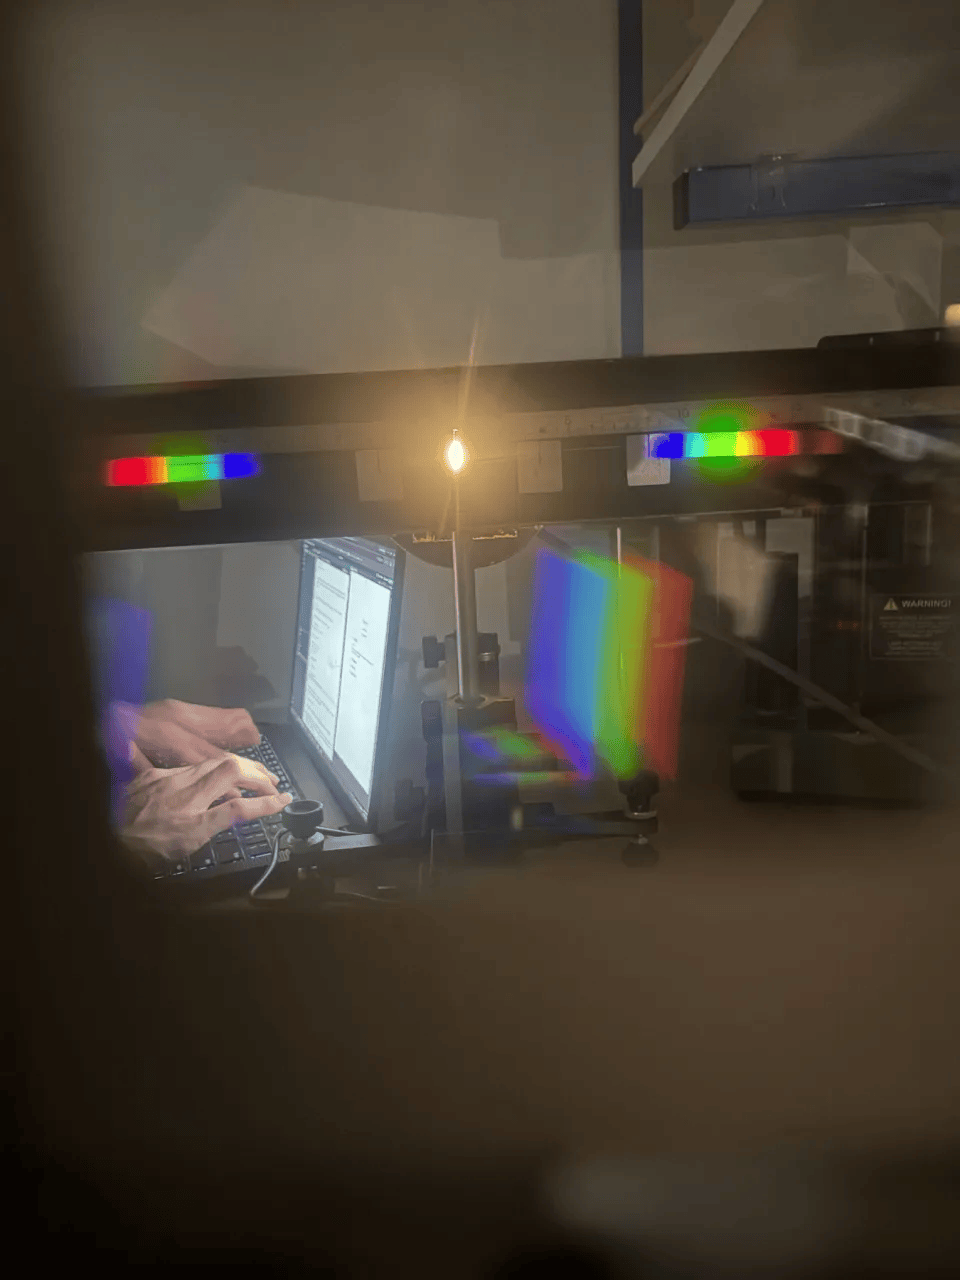
\includegraphics[width=\linewidth,trim=80bp 700bp 80bp 300bp,clip]{Photos/5CL_5_4b.png}
\caption{The smoother spectrum of the incandescent bulb.}
\end{figure}

\clearpage

\end{document}
